% ---------------------------------------------------------------------------
% Author guideline and sample document for EG publication using LaTeX2e input
% D.Fellner, v1.13, Jul 31, 2008

\documentclass{egpubl-eurovis-star}
\usepackage{eurovis2014-star}

% --- for EuroVis
%\WsSubmission    % uncomment for submission to EuroVis
\WsPaper         % uncomment for final version of EuroVis contribution

\electronicVersion % can be used both for the printed and electronic version

% !! *please* don't change anything above
% !! unless you REALLY know what you are doing
% ------------------------------------------------------------------------

% for including postscript figures
% mind: package option 'draft' will replace PS figure by a filname within a frame
\ifpdf \usepackage[pdftex]{graphicx} \pdfcompresslevel=9
\else \usepackage[dvips]{graphicx} \fi

\PrintedOrElectronic

% prepare for electronic version of your document
\usepackage{t1enc,dfadobe}

\usepackage{egweblnk}
\usepackage{cite}

% For backwards compatibility to old LaTeX type font selection.
% Uncomment if your document adheres to LaTeX2e recommendations.
% \let\rm=\rmfamily    \let\sf=\sffamily    \let\tt=\ttfamily
% \let\it=\itshape     \let\sl=\slshape     \let\sc=\scshape
% \let\bf=\bfseries

% end of prologue

%\input{EGauthorGuidelines-body.inc} % commented by KK for ShareLaTeX use

% ---------------------------------------------------------------------
% EG author guidelines plus sample file for EG publication using LaTeX2e input
% D.Fellner, v1.17, Sep 23, 2010


\title[EG \LaTeX\ Author Guidelines]%
      {Bridge and terrain reconstruction in LiDAR point clouds}

% For anonymous conference submission, please enter your SUBMISSION ID.
\author[submission ID]{Timotej Kovač}

%% For the final version of your accepted paper, please enter the authors names and affiliations.
%\author[D. Fellner \& S. Behnke]
%       {D.\,W. Fellner\thanks{Chairman Eurographics Publications Board}$^{1,2}$
%        and S. Behnke$^{2}$
%        \\
%         $^1$TU Darmstadt \& Fraunhofer IGD, Germany\\
%         $^2$Institut f{\"u}r ComputerGraphik \& Wissensvisualisierung, TU Graz, Austria
%       }

% ------------------------------------------------------------------------

% if the Editors-in-Chief have given you the data, you may uncomment
% the following five lines and insert it here
%
% \volume{27}   % the volume in which the issue will be published;
% \issue{1}     % the issue number of the publication
% \pStartPage{1}      % set starting page


%-------------------------------------------------------------------------
\begin{document}

% \teaser{
%  
\includegraphics[width=\linewidth]{eg_new}
%  \centering
%   \caption{New EG Logo}
% \label{fig:teaser}
% }

\maketitle

\begin{abstract}
When LiDAR data of the terrain is being acquired some object might interfere with the surroundings in such a way that a lot of detail is lost.
One type of these interference objects are bridges.
Details of them are lost and they are in the way of capturing on the terrain bellow.
In this paper we propose an algorithm to reconstruct the lost terrain bellow them and also their reconstruction using additional data.
We discuss the results that this kind of an approach brings and what can be done to further improve it.
\end{abstract}



\section{Introduction}
In this paper we discuss a possible approach to reconstruct bridges and terrain undernthem.
We also discuss how the additional data in the form of SHP files which were available to us from the e-Geodetski podatki web site proved effective in our algorithm.~\cite{shp, egeodetskipodatki}.
These contain geometries and some basic information about infrastructure such as bridges and natural resources such as rivers.
We also show the results that we produced using some a simple interpolation approach, our own approach and the final result of the reconstruction process.

\section{Implementation}
For our tests we have chosen a very complex bridge example in order to make our approach as robust as possible.
Our example consisted of two adjecent bridges that extended over a moving body of water at an angle that wasn't perpendicular to it.
Both also extended over a large portion of the terrain.

Our implementation was done in Java with the help of libraries LASzip and GeoTools libraries which were used for reading the LAZ and SHP files.~\cite{lasreader, geotools}.

\subsection{Bridge reconstruction}

Because of the nature of how the LiDAR data is gathered the surface bellow the bridge is missing.
To reconstruct this part of the bridge we used the additional data about the bridges location and width to determine 4 keypoints that defined that bridge.
In reality bridges can be more complicated and composed of multiple bridge segments so our approach was to determine the keypoints on the particular bridge segment and at the end these would be groupped together to form a final result.
Using this approach we gained the x and y values of each of the defining vertices of the bridge and so had to interpolate the z coordinate.
This was done using either finding enough low value points (based on the z component) that were classified as being part of the bridge.
These also had to be in some determined range to be deemed valid.
After that the z-component was calculated as an interpolation with weight in regards to distance from the point we wanted to interpolate and other points that matched the above criteria.
Then we simply interpolated withing these four points the ones that defined the bridge bottom.

\subsection{Terrain reconstruction}


The majority of our effort was aimed towards reconstructing the surface underneath the bridge.

At the start we tried some basic approaches towards terrain reconstruction and got some insight into problems that we will have to solve.
These were:
\begin{itemize}
\item{how to generate points on this area to best reconstruct the terrain and}
\item{how to deal with outliers, vegetation, power lines and object that are adjecent to bridges and don't represent the terrain.}
\end{itemize}

Our approach can be seen on figure~\ref{fig2} and is described bellow.
\begin{figure}[ht]
    \centering
    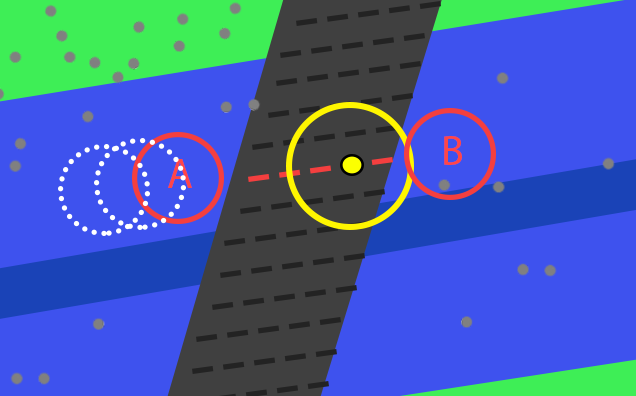
\includegraphics[width=1\columnwidth]{bridge.png}
    \caption{ }
    \label{fig2}
\end{figure}
\begin{enumerate}
\item{Define the bridge polygon from the SHP file and temporary remove every point that is determined to belong to a bridge.}
\item{Generate values x and y along the bridge in such a way that they run parallel to the valley bellow the bridge. }
\item{Sample points from both sides of this line (terrain adjecent to the bridge marked with A and B). 
If there are too few points sampled then continue searching in the same direction until some threshold (white dotted circle).
If there are still not enough points to be found sample the surrounging area of the terrain that has already been completed (yellow circle).}
\item{Process the sampled points to remove any objects that aren't terrain.}
\item{Interpolate the z coordinate with distance as a weight on sampled points.}
\end{enumerate}

\section{Results}

Our first attempt at solving this issue can be seen as the red part of the figure~\ref{fig1}.
\begin{figure}[ht]
    \centering
    
\includegraphics[width=1\columnwidth]{terrain_inter.png}
    
\includegraphics[width=1\columnwidth]{terrain_br.png}
    \caption{Results of terrain reconstruction. Image in red shows the closest neighbour interpolation while the blue image shows selected group interpolation.}
    \label{fig1}
\end{figure}

Here we used a simple approach of a weighted nearest neigbour interpolation. 
As it can be seen reconstructed points do not follow the reality of the terrain well.
The majority of points are interpolated to roughly the right height but the transitions between them are very harsh.

Our approach on the other hand gave us very good results in reconstructing the terrain under a bridge and can be seen drawn in blue in the same figure ~\ref{fig1}.
The whole reconstruction process of the bridge and terrain on an example of two highway bridges produced the results in under half a minute, but this may vary depending on the system used and number and complexity of bridges.
The cloud points before and after the reconstruction process can be seen in figures ~\ref{fig3} and ~\ref{fig4}.
In them the added points of the bottom bridge and the reconstruction of the bottom of the river under the bridge and its banks can be clearly seen.

\begin{figure}[ht]
    \centering
    
\includegraphics[width=1\columnwidth]{side_pre_3.png}
    
\includegraphics[width=1\columnwidth]{side_br_3.png}
    \caption{Results of terrain and bridge reconstruction. Image in yellow shows the original data while the blue image shows the added reconstructed data.}
    \label{fig3}
\end{figure}

\begin{figure}[ht]
    \centering
    
\includegraphics[width=1\columnwidth]{front_pre.png}
    
\includegraphics[width=1\columnwidth]{front_br.png}
    \caption{Results of terrain and bridge reconstruction. Image in yellow shows the original data while the blue image shows the added reconstructed data.}
    \label{fig4}
\end{figure}


\section{Further work}

One of the issues we didn't solve is that of saving the reconstructed data in LAZ format.
We weren't sucessful in finding any free library that we could use to save the reconstructed data in the same LAZ format as the input file.
That is why the system outputs a simple OBJ file which contains the reconstructed bridge points alongside with the original points inside of a certain circumference of the bridge.

Another issue we had and didn't manage to solve was that of bridge, road and river intersections.
For our approach it was crucial that we detected which bridges, roads and rivers intersected where, so that we could paired them and calculated the normals used for terrain and bridge reconstruction.
Roads were needed to get the width of the bridge, as that wasn't specified in the bridges SHP file.
Because of that we had to manually open 3 different SHP files and gathered the required information out of each one.
The road that is on the bridge and the bridge itself were in two different SHP files and even though they supposedly all use the D48/GK koordinate system the values didn't match up~\cite{d48gk}.
When trying to solve this by converting objects in their coordinate systems into a common one the problem still persisted.
We approached this problem by manually extracting the IDs of bridges, roads and rivers from the different SHP files and then only searching among those.
This isn't the best solution as manually extracting IDs is a tideous task but neverthelesss for our purpouses we went with this approach.
If this was fixed however one would just need to uncomment the code for intesections and this problem would be solved, as we did implement the correct way of merging these various objects.

More of the infrastructure of terrain bellow the bridge could also be supported.
For now only rivers have been supported but also roads, railways or any other kind of infrastructure could be supported as well with the right SHP files and filtering attributes.

\section{Conclusion}

We were sucessful in implementing a rather robust approach for reconstructing bridges and terrain underneath.
The reconstruction algorhitm is aware of the natural flow of the terrain and the points that are important for interpolation.
Compared to simple interpolation methods our approach provided better results while still giving the result in an acceptable amount of time.
Further work could be done improving this approach especially on reconstructing the bridge.

%\bibliographystyle{eg-alpha}
\bibliographystyle{eg-alpha-doi}

\bibliography{egbibsample}

\end{document}

